% !TEX program = xelatex
% 论文主文档：汇总章节、参考文献与附录。
% 正文内容请到 sections/ 下按章节编辑，避免多人同时改本文件。

\PassOptionsToPackage{quiet}{xeCJK}
\documentclass[withoutpreface,bwprint]{cumcmthesis}

% ================= 宏包与格式 =================
\makeatletter
% 正文改五号(10.5pt), 行距 12.0pt*1.38 ~ 16.6pt, 与参考论文格式一致
\renewcommand\normalsize{\@setfontsize\normalsize{10.5}{12.0}}
\makeatother
\geometry{top=25mm,bottom=20mm,left=20mm,right=20mm}
\usepackage{etoolbox}
\usepackage{ctex}
\usepackage{graphicx}   % 插图（\includegraphics 必需）
\usepackage{booktabs}   % 三线表（\toprule\midrule\bottomrule）
\usepackage{amsmath}    % 数学公式环境（equation 等）
\BeforeBeginEnvironment{tabular}{\zihao{-5}}
\usepackage[numbers,sort&compress]{natbib}   % 参考文献
\usepackage[framemethod=TikZ]{mdframed}      % 框架
\usepackage{url}
\usepackage{subcaption}                      % 子图
\newcolumntype{C}{>{\centering\arraybackslash}X}
\newcolumntype{R}{>{\raggedleft\arraybackslash}X}
\newcolumntype{L}{>{\raggedright\arraybackslash}X}
\renewcommand{\textbf}[1]{{\song\bfseries #1}}

% 流程图样式（技术路线图等可用）

% 流程图样式（技术路线图等可用）
\usepackage{tikz}
\usetikzlibrary{calc}
\usetikzlibrary{shapes.geometric, arrows.meta, positioning}
\tikzstyle{startstop}=[rectangle, rounded corners, minimum width=3cm, minimum height=1cm, text centered, draw=black, fill=red!20]
\tikzstyle{process}=[rectangle, minimum width=3.5cm, minimum height=1cm, text centered, draw=black, fill=blue!20]
\tikzstyle{decision}=[diamond, aspect=2, minimum width=3.5cm, minimum height=1cm, text centered, draw=black, fill=green!20]
\tikzstyle{arrow}=[thick,->,>=stealth]

% ================= 论文基本信息 =================
\title{数据驱动的蔬菜类商品自动定价与补货决策建模}

\begin{document}

\pagenumbering{gobble}   % 封面、目录不显示页码
\maketitle

% 摘要：比赛最后统一定稿，由负责统稿的同学维护。
\begin{abstract}

\textbf{针对问题一：}待写。

\textbf{针对问题二：}待写。

\textbf{针对问题三：}待写。

\textbf{针对问题四：}待写。

\keywords{关键词1；关键词2；关键词3；关键词4；关键词5}

\end{abstract}


% \tableofcontents        % 需要目录时取消注释

\pagenumbering{arabic}
% 问题重述与分析
\section{引言}
\subsection{问题背景}
生鲜商超是城市居民日常消费的重要渠道，其中蔬菜类商品因消费频率高、需求刚性强的特点，在商超经营中占据关键地位。然而，蔬菜类商品保鲜期短、品相变化快，商超需按日进行补货。并且，由于蔬菜品种与产地繁多，且进货交易时间集中在凌晨3:00至4:00，商超往往在信息不完全的情况下做出当日补货决策。同时，蔬菜类商品在需求侧呈现出销售量与时间关联关系，在供给侧中则表现出季节性，以及与销售空间限制的紧密联系。在此背景下，如何依据历史销售数据、批发价格和损耗率等信息，科学制定蔬菜类商品的补货、定价、销售组合策略，已成为生鲜商超经营管理的核心问题之一。

\subsection{问题重述}
本题基于某商超经销的6个蔬菜品类的商品信息（附件1）、2020年7月1日至2023年6月30日的销售流水明细数据（附件2）与批发价格数据（附件3），以及各商品近期的损耗率数据（附件4），解决以下四个问题：

\textbf{问题一：}要求基于附件1、2等数据来源，分析各蔬菜品类及单品在销售量上的分布规律，如时间分布特征（季节性、周期性等），并揭示相关关系，如不同品类之间、不同单品之间可能存在的互补或替代关系，为后续补货与定价决策提供依据。

\textbf{问题二：}要求基于附件1、2、3、4等数据来源，在品类层面上建立销售总量与成本加成定价之间的关系模型，并在此基础上确定未来一周（2023年7月1日至7日）日补货总量和定价策略，以最大化商超的总收益。

\textbf{问题三：}要求基于附件2等数据来源，在可售单品总数控制在27至33个，且各单品订购量满足最小陈列量2.5千克的基础下，根据2023年6月24日至30日的可售品种，制定7月1日的单品补货量和定价策略，在尽量满足市场需求前提下，使得商超收益最大。

\textbf{问题四：}要求从优化制定蔬菜类商品补货和定价决策的角度出发，识别当前数据体系的不足，提出补充采集数据的意见和理由，并论述这些数据如何帮助解决上述问题。

\subsection{问题分析}

\textbf{问题一：}属于统计规律刻画与关联结构识别问题。以附件1（6品类、251单品）与附件2（2020-07-01至2023-06-30销售流水，$T=1095$天）为输入，输出品类与单品的销量分布形态、时间特征及协同关联。三个统计事实决定建模路径：(1)品类日销量为连续正值、右偏长尾，用对数正态/伽马分布拟合，AIC/BIC选型；(2)单品日销量存在大量无销售日，采用“售出概率$+$正销量条件分布”的两阶段混合模型；(3)原始日销量相关混入共同日历与季节成分会产生伪相关\cite{yule1926}，须先剔除时间效应再构建关联网络；单品销售形态差异悬殊，以时序特征聚类分组。据此拆解为分布拟合、STL季节分解、去季节关联网络、时序特征聚类四个子模型。

\textbf{问题二：}属于品类层面的关系建模与随机优化决策问题。要求刻画销售总量与成本加成定价的关系（Log-Log弹性回归），并给出未来一周各品类的日补货总量与定价策略使收益最大。三个难点决定模型结构：(1)价格与销量的内生性：须先界定品类售价口径；(2)时序约束：最优加价率$m_c^*$只依赖品类弹性与损耗率、与批发价无关；(3)需求随机与损耗：按报童临界比$\kappa=(P^*-c')/P^*$在缺货与损耗间权衡。按“弹性回归$\to$最优定价$\to$去价格需求预测$\to$报童补货”四步建模，批发价以最近一周均价估计。

\textbf{问题三：}属于单品级联合组合优化问题。以2023-06-24至30可售品种为候选，同时决策单品是否上架、选哪档价、订多少货，满足可售总数27--33、单品最小陈列量2.5kg的耦合约束。与问题二相比：(1)决策粒度由品类下放到单品；(2)跨单品共享约束使问题无法按品类独立优化\cite{kok2009,vanryzin1999}。三个对策：(1)单品弹性借用品类弹性先验做Shrinkage估计\cite{james1961}；(2)售价离散为$K=11$档价格网格，转化为线性0-1 MIP保证全局最优\cite{wolsey1998}；(3)以缺货惩罚软约束量化“满足需求”，配合灵敏度给出权衡\cite{khouja1999}。模型复用问题一的聚类分组与问题二的弹性、损耗参数。

\textbf{问题四：}属于数据体系诊断与采集方案建议问题。从优化补货定价决策出发，识别现有数据不足，提出补充采集建议。基于建模过程定位五类缺失：(1)日销量聚合口径无法区分共同趋势与真实关联，购物篮关系不可识别；(2)售价口径混合正常销售与打折价，弹性向零衰减；(3)缺货日真实需求不可观测；(4)损耗率为静态均值、缺乏动态结构；(5)数据粒度为日级，缺少日内信息与外部竞品参照。据此从需求侧、市场侧、运营侧、供给侧与外部环境五个维度提出采集方案，每条按“补什么数据—改进哪个模型—改善哪个指标”的链条与前文挂钩。
% 模型假设与符号说明
\section{模型假设}
为简化问题，本文做出以下假设：
\begin{itemize}[itemindent=2em]
  \item 假设1：待写。
  \item 假设2：待写。
  \item 假设3：待写。
\end{itemize}

\section{符号说明}
\begin{table}[H]
  \centering
  \begin{tabularx}{\textwidth}{CL}
    \toprule
    符号 & 说明 \\
    \midrule
    $x$ & 待写 \\
    \bottomrule
  \end{tabularx}
  \caption{符号说明}
  \label{tab:符号说明}
\end{table}

% 问题一
\section{问题一的模型建立与求解}
\subsection{问题分析}
待写。

\subsection{模型准备}
待写。

\subsection{模型建立}
待写。

\subsection{模型求解与结果分析}
待写。

% 问题二
\section{问题二的模型建立与求解}

\subsection{模型准备}

\subsubsection{数据来源与整合}

本问使用附件 1–4：品类日销量 $Q_{c,t}$、品类加权售价 $P_{c,t}$ 与批发价 $W_{c,t}$ 在附件 2、3 基础上沿用问题一的清洗与聚合口径构建（退货以负销量并入净销量），损耗率 $L_c$ 由附件 4 单品损耗率按固定销量份额加权聚合。

\subsubsection{统计口径}

关键量的统计口径如表 \ref{tab:q2_stats} 所示。

\begin{table}[htbp]
\centering
\caption{问题二统计口径}
\label{tab:q2_stats}
\begin{tabular}{cll}
\toprule
量 & 口径 & 来源 \\
\midrule
$Q_{c,t}$ 品类日净销量 & 附件 2 按单品—品类映射聚合，退货以负销量并入当日净销量 & 附件 2 \\
$W_{c,t}$ 品类批发价 & 附件 3 单品批发价按固定基期销量份额加权 & 附件 3 \\
$L_c$ 品类损耗率 & 附件 4 单品损耗率按固定销量份额加权：$L_c=\sum_i w_i L_i$（百分数，代入公式前除以 100） & 附件 4 \\
$P_{c,t}$ 品类售价 & 单品售价按\textbf{固定基期销量权重}加权（Laspeyres 型价格指数） & 附件 2 \\
\bottomrule
\end{tabular}
\end{table}

\subsection{模型建立}
\label{sec:q2_model}

\subsubsection{需求—价格关系：品类 Log-Log 弹性回归}

对品类 $c$ 建立双对数（常弹性）回归：
\begin{equation}
\ln Q_{c,t}=\alpha_c+\beta_c\ln P_{c,t}+\delta_c\,t+\sum_{k=1}^{6}\delta_{c,k}\,\mathbb{1}_{\{\mathrm{weekday}=k\}}+\sum_{m=1}^{11}\eta_{c,m}\,\mathbb{1}_{\{\mathrm{month}=m\}}+\varepsilon_{c,t},
\end{equation}
其中 $\beta_c$ 为价格弹性（预期为负），$t$ 为线性趋势项（防止伪回归），星期虚拟变量（基准周一）与月份虚拟变量（基准 1 月）刻画周期结构，$\delta_{c,k}$、$\eta_{c,m}$ 分别为星期与月份虚拟变量系数，记号与问题一残差回归（$\delta_k$、$\eta_m$）一致。双对数形式的优点在于弹性为常数，可直接外推“销量—价格”反事实，是销量—价格实证研究的标准形式 \cite{tellis1988}。

每个品类独立做 OLS 估计，报告弹性 $\hat\beta_c$、$t$ 值（显著性）、$R^2$ 与样本量，并做残差平稳性（DW/ADF）检验防止伪回归 \cite{wooldridge2010}。内生性处理上，价格与当期需求同时决定，OLS 可能有偏，稳健性做法是用滞后一期价格 $\ln P_{c,t-1}$ 替代当期价格重新估计，或采用工具变量，论文报告两种估计的差异作为稳健性证据 \cite{wooldridge2010}。销量截断方面，缺货日的销量低估真实需求，若缺货与价格相关（如低价日需求更高、更易缺货），弹性估计会受截断影响，作为局限写入小结。

价格口径与加价率的衔接：由于售价 $P=(1+k)W$，在控制批发价 $\ln W$ 后，$\ln(1+k)$ 的系数即 $\beta_c$，即“批发价不变时，加价率弹性等于价格弹性”，故 $\beta_c$ 同时刻画“销售总量对成本加成加价率”的敏感程度；反事实示例需注明“批发价不变”。

\subsubsection{最优定价：成本加成加价率解析解}

\textbf{有效进货成本}。损耗率 $L_c$ 表示进货量中最终损耗的比例，售出 1 kg 需进货 $1/(1-L_c)$ kg，故单位售出成本为 \cite{nahmias1982,blackburn2009,tang2018}
\begin{equation}
c'_{c,t}=\frac{W_{c,t}}{1-L_c}.
\end{equation}
注意附件 4 的损耗率为百分数（如 12.83 表示 12.83\%），代入上式前需除以 100，否则有效成本为负、临界比越界。

\textbf{常弹性最优加价率}。在参考点 $(\bar Q_c,\bar P_c)$ 处把需求近似为常弹性函数 $Q(P)=\bar Q_c(P/\bar P_c)^{\beta_c}$，单日利润为 \cite{petruzzi1999}
\begin{equation}
\pi(P)=\left(P-c'_{c,t}\right)\bar Q_c\left(\frac{P}{\bar P_c}\right)^{\beta_c}.
\end{equation}
对 $P$ 求导并令导数为零（记 $E_c=|\beta_c|>1$ 时为极大值）：
\begin{equation}
\frac{d\pi}{dP}=\bar Q_c\left(\frac{P}{\bar P_c}\right)^{\beta_c}\left[1+\beta_c\frac{P-c'_{c,t}}{P}\right]=0 \quad\Longrightarrow\quad P^*_{c,t}=\frac{E_c}{E_c-1}\,c'_{c,t}=\frac{E_c}{E_c-1}\cdot\frac{W_{c,t}}{1-L_c}.
\end{equation}
对应批发价加价率（即“成本加成”倍率）为
\begin{equation}
m^*_c=\frac{P^*_{c,t}}{W_{c,t}}-1=\frac{E_c}{(E_c-1)(1-L_c)}-1.
\end{equation}
该式等价于垄断定价的逆弹性规则（Lerner 条件）$(P^*-c')/P^*=1/E_c$ \cite{mascolel1995}，且解析最优价处报童临界比恰为 $\kappa^*=(P^*-c')/P^*=1/E_c$，与 \ref{sec:newsvendor} 节衔接。

需说明：$\kappa^*=1/E_c$ 仅在解析最优解处成立；本问各品类弹性均小于 1、落入数值求解分支（\ref{sec:result}节），临界比一律按定义 $\kappa=(P^*-c')/P^*$ 直接计算（表 \ref{tab:q2_pricing}），不直接使用该关系。

\textbf{关键性质与决策规则}：$m^*_c$ 只依赖弹性与损耗率、与批发价 $W_{c,t}$ 无关。因此商超可在凌晨未知当日批发价时预先确定品类加价率策略，到货后按实际批发价确定售价 $P^*_{c,t}=(1+m^*_c)W_{c,t}$——这既对应题面“成本加成定价”，也化解了“凌晨 3:00–4:00 不知具体进货价”的时序约束。

\textbf{边界处理与数值求解}：

\begin{enumerate}
\item 若历史估计 $E_c\le 1$（无弹性或弱弹性），解析解不存在或无最大值，改在历史加价率百分位区间 $[m_{5\%},m_{95\%}]$ 内以 201 点等距网格数值搜索最优加价率 \cite{tellis1988}；
\item 网格搜索中利润一律按\textbf{截断后的最终售价} $P=\min(\max((1+k)W,P_5),P_{95})$ 评估，需求仍以最终售价为自变量，避免“评估价与最终售价脱节”；
\item 解析解分支同样将最优价截断在历史价格区间 $[P_5,P_{95}]$ 内，防止常弹性外推越界；
\item 输出中标注各品类弹性 $E_c$、加价率 $m^*_c$ 及是否命中解析解，保证可追溯。
\end{enumerate}

\textbf{说明}：当 $E_c<1$ 时利润函数在可行加价率区间内单调递增，网格最优落在可行域边界——多数品类为加价率上界 $m_{95\%}$，花菜类与水生根茎类受价格上界 $P_{95}$ 约束（见9.1节）；论文中的最优加价率应理解为“\textbf{历史交易区间约束下的最优}”，而非无条件全局最优，区间边界敏感性见 \ref{sensitivity_analysis} 节。

\subsubsection{基准需求预测：去价格序列 + 趋势—周期外推}

\textbf{去价格变换}。先用第 \ref{sec:q2_model} 节估计的弹性 $\hat\beta_c$ 把历史销量折算到统一参考价 $\bar P_c$（取历史加权均价）下的“无价格效应需求”：
\begin{equation}
Q^0_{c,t}=Q_{c,t}\left(\frac{\bar P_c}{P_{c,t}}\right)^{\hat\beta_c}.
\end{equation}
因 $\hat\beta_c<0$，历史价高于参考价的日子需求被上调、低于参考价的日子被下调，序列 $Q^0$ 保留趋势/星期/季节结构但剔除价格影响。\textbf{若不先剔除价格效应就直接预测原始销量、再乘价格比，价格效应会被重复计入} \cite{taylor2018,hyndman2018}。

\textbf{外推预测}。对去价格序列 $Q^0_{c,t}$ 建模并外推未来一周参考价下的基准需求 $\bar Q_{c,t}$ 与残差标准差 $\sigma_{c,t}$（模型设计以 Prophet 为基准，含周与年季节项；代码实现为等价的含线性趋势、星期与月份虚拟变量的回归外推，并对数均值修正，即 $\bar Q=\exp(\widehat{\ln Q}+\mathrm{MSE}/2)$、$\sigma=\bar Q\sqrt{\exp(\mathrm{MSE})-1}$，两种实现等价 \cite{taylor2018,hyndman2018}）。

\textbf{最优定价下的需求分布（乘性缩放）}。在最优售价 $P^*$ 下，需求按弹性整体缩放（乘性需求假设，是定价—报童联合问题的标准设定 \cite{petruzzi1999}）：
\begin{equation}
\mu_{c,t}(P^*)=\bar Q_{c,t}\left(\frac{P^*_{c,t}}{\bar P_c}\right)^{\hat\beta_c},\qquad \sigma_{c,t}(P^*)=\sigma_{c,t}\left(\frac{P^*_{c,t}}{\bar P_c}\right)^{\hat\beta_c}.
\end{equation}
假设含义：价格只改变需求水平、不改变变异系数，分布形态随价格同比例缩放；该假设已在模型假设中说明。

\subsubsection{报童补货模型}
\label{sec:newsvendor}

设进货可售量 $y=(1-L_c)R$，需求分布为 $F$（均值为 $\mu$、标准差为 $\sigma$、价格为 $P^*$），单位售出成本 $c'=W/(1-L_c)$，残值为 0。报童模型的最优条件对任意需求分布成立 \cite{silver2016,khouja1999,petruzzi1999}：
\begin{equation}
E\pi=P^*\cdot E[\min(D,y)]-c'\cdot y.
\end{equation}
最优可售量满足分位数条件 $F(y^*)=\kappa_{c,t}$，临界比为
\begin{equation}
\kappa_{c,t}=\frac{P^*_{c,t}-c'_{c,t}}{P^*_{c,t}}=\frac{P^*_{c,t}-W_{c,t}/(1-L_c)}{P^*_{c,t}}.
\end{equation}

\textbf{分布口径与问题一衔接}：问题一按 AIC 为各品类从伽马、对数正态两类右偏连续分布中选择拟合（花叶类、花菜类、水生根茎类、茄类为伽马，辣椒类、食用菌为对数正态）。为与代码实现一致，本问统一采用对数正态矩匹配分位数作为实现口径：由预测期均值 $\mu$ 与标准差 $\sigma$ 矩匹配对数参数（$\mu_{\ln}=\ln\left(\mu^2/\sqrt{\mu^2+\sigma^2}\right)$、$\sigma_{\ln}=\sqrt{\ln\left(1+\sigma^2/\mu^2\right)}$）后计算 $y^*=\exp\left(\mu_{\ln}+\sigma_{\ln}\,\Phi^{-1}(\kappa)\right)$，伽马与对数正态分位数之差并入近似误差。
\begin{equation}
y^*_{c,t}=\mu_{c,t}(P^*)+\sigma_{c,t}(P^*)\,z_c(\kappa_{c,t}),
\end{equation}
其中 $z_c(\kappa)=F_c^{-1}(\kappa)$ 为品类 $c$ 拟合分布标准化后的 $\kappa$ 分位数；不依赖参数分布时，用历史残差的经验分位数 $\hat F^{-1}(\kappa)$ 替代 \cite{agrawal1996}。每日品类补货总量为
\begin{equation}
R_{c,t}=\frac{y^*_{c,t}}{1-L_c}=\frac{\mu_{c,t}(P^*)+\sigma_{c,t}(P^*)\,z_c(\kappa_{c,t})}{1-L_c}.
\end{equation}

说明：
\begin{itemize}
\item 正态分布只是 $z_c(\kappa)=\Phi^{-1}(\kappa)$ 的特例；右偏分布下同一 $\kappa$ 的分位数与正态明显不同（如 $\kappa=0.5$ 时正态给均值、lognormal 给中位数），故统一采用对数正态矩匹配分位数，正态仅作近似对比 \cite{agrawal1996}；
\item $z_c(\kappa)<0$ 表示“负安全库存”，即可售量 $y^*$ 低于需求均值 $\mu(P^*)$。对右偏分布均值高于中位数，$z_c(\kappa)<0$ 的临界 $\kappa$ 大于 0.5；本问 6 品类临界比均小于 0.5，均处于“负安全库存”区域——需求波动大且超量损耗成本高时，以适度缺货风险换取更低的超量损耗成本，属报童最优条件的正常结果；
\item 除以 $(1-L_c)$ 是把可售量折算回进货量，补偿损耗 \cite{nahmias1982}；
\item 口径局限：问题一拟合的是已售销量而非真实需求，缺货日销量低估需求，报童补货量可能系统性偏低。
\end{itemize}

确定性对照：忽略需求波动（$z_c=0$）时的补货量为 $R^0_{c,t}=\mu_{c,t}(P^*)/(1-L_c)$，作为“无安全库存”基准。

\subsubsection{品类独立优化的合理性：相关性只进入方差、不进期望}

问题一识别出品类销量存在协同变动，本节论证逐品类独立定价与补货不损失期望利润。记品类 $c$ 的期望利润 $f_c(R_c)=E_{D_c}\left[\pi_c(R_c;D_c)\right]$，其只依赖品类 $c$ 自身的边际需求分布 $F_c$（$\pi_c$ 中不含其他品类的销量或价格）。

\textbf{命题 1（期望可加与可分最大化）}：期望的线性性给出 $E[\sum_c\pi_c]=\sum_c E[\pi_c]$；又因每个 $f_c$ 只含自己的决策 $R_c$ 且可行集可分，最大化的“和”可逐项分解：
\begin{equation}
\max_{R\in X}\sum_{c=1}^{6}f_c(R_c)=\sum_{c=1}^{6}\max_{R_c\in X_c}f_c(R_c).
\end{equation}
该分解性是多品无约束报童问题的标准结论：无容量约束时，多品报童退化为相互独立的单品问题 \cite{silver2016}。

\textbf{命题 2（最优订货只依赖边际分布）}：报童最优条件 $F_c(y^*_c)=\kappa_c$ 只含品类 $c$ 的边际 CDF。品类间相关性刻画的是联合分布结构，不改变任何一个边际分布 $F_c$，故不改变任一品类的最优订货量 $y^*_c$ 与补货量 $R^*_c$（单周期报童模型的基本性质 \cite{khouja1999,petruzzi1999}）。

\textbf{推论}：在风险中性假设下（题面“收益最大”即指最大化期望利润），逐品类独立优化与整体联合优化的最优决策相同。协方差矩阵既不进入临界比条件（\ref{sec:newsvendor}节），也不进入最优价公式（\ref{sec:q2_model}节），最优补货量与最优售价均与品类间相关性无关；相关性只进入总利润的方差分解：
\begin{equation}
\mathrm{Var}\left(\sum_c\pi_c\right)=\sum_c\mathrm{Var}(\pi_c)+2\sum_{c<c'}\mathrm{Cov}(\pi_c,\pi_{c'}).
\end{equation}
正相关通过协方差项放大总利润波动，但不改变期望利润（组合理论的基本结论 \cite{markowitz1952}）。

\textbf{结论成立的三项条件}：
\begin{enumerate}
\item 目标可加：各品类利润函数互不包含（本模型需求函数无交叉价格项）；
\item 决策集可分：无共享资金、货架或订货容量约束（问题二成立，问题三不成立）；
\item 边际分布外生：品类 $c$ 的需求边际分布不受其他品类定价决策的影响。
\end{enumerate}

\textbf{失效情形与本文定位}：若商超风险厌恶或存在联合风险约束（资金预算、亏损概率上限），利润联动会改变最优决策 \cite{chen2009}；存在共享容量约束，需联合优化 \cite{abdelmalek2004}；需求存在替代/互补（涨价导致跨品类转移），独立定价不是真实意义上的全局最优。其中 ③ 最贴近本题现实：问题一的相关性分析只能识别“销量同步变动”，不能识别因果替代结构，交叉价格弹性建模留待问题四的数据扩展；本文在 \ref{stability_q2} 节用交叉价格弹性联合定价模拟作为稳健性对照。


\subsection{模型求解与结果分析}
\label{sec:result}

\subsubsection{弹性估计结果}

对 6 个品类分别估计 Log-Log 回归，结果如表 \ref{tab:q2_elasticity} 所示（样本期 1095 天，$n$ 为各品类正销量日样本量；参考价为历史加权均价，参考需求为正销量日均值）。

\begin{table}[htbp]
\centering
\caption{品类价格弹性与定价参数}
\label{tab:q2_elasticity}
\begin{tabular}{lccccccccccc}
\toprule
品类 & 价格弹性 $\hat\beta_c$ & $t$ 值 & $R^2$ & 样本量 $n$ & 参考价 $\bar P_c$（元/kg） & 参考需求 $\bar Q_c$（kg） & 有效成本 $c'$（元/kg） & 加价率 $m_{5\%}$ & 加价率 $m_{95\%}$ & 最优加价率 $m^*_c$ & 是否解析解 \\
\midrule
花叶类 & -0.45 & -6.79 & 0.40 & 1085 & 5.89 & 183.22 & 4.11 & 0.44 & 1.01 & 1.01 & 否 \\
花菜类 & -0.50 & -5.45 & 0.31 & 1084 & 9.95 & 38.57 & 9.69 & 0.27 & 0.79 & 0.71 & 否 \\
水生根茎类 & -0.07 & -0.70 & 0.61 & 1085 & 9.22 & 37.45 & 12.93 & 0.26 & 0.70 & 0.44 & 否 \\
茄类 & -0.26 & -3.16 & 0.52 & 1050 & 8.80 & 21.38 & 4.41 & 0.30 & 0.90 & 0.90 & 否 \\
辣椒类 & -0.13 & -3.03 & 0.45 & 1085 & 8.63 & 84.52 & 3.49 & 0.26 & 1.14 & 1.14 & 否 \\
食用菌 & -0.31 & -5.28 & 0.41 & 1085 & 11.09 & 70.21 & 2.76 & 0.35 & 0.82 & 0.82 & 否 \\
\bottomrule
\end{tabular}
\end{table}

解读如下：

\begin{itemize}
\item 全部品类的价格弹性均为负，其中花叶类（-0.45）、花菜类（-0.50）需求价格敏感度最高，水生根茎类（-0.07）几乎无价格弹性；除水生根茎类（$t=-0.70$，不显著）外，其余品类弹性均在 1\% 水平显著；
\item 由于“批发价不变时加价率弹性等于价格弹性”（\ref{sec:q2_model}节），表 \ref{tab:q2_elasticity} 的 $\hat\beta_c$ 即销售总量对成本加成加价率的敏感度：花叶类加价率每提高 1\%，销量约下降 0.45\%；
\item \textbf{所有品类 $E_c=|\beta_c|<1$，均不满足解析解条件}，表 \ref{tab:q2_elasticity} 的最优加价率均为“历史加价率区间 $[m_{5\%},m_{95\%}]$ 网格 201 点的数值最优”，即历史区间约束下的最优，而非无条件解析最优；
\item 水生根茎类弹性不显著，其定价结论的证据强度相应降低，加价率主要由历史区间约束决定，需谨慎解读。
\end{itemize}

\begin{figure}[htbp]
\centering

\includegraphics[width=0.9\textwidth]{../figures/q2_elasticity_fit.pdf}
\caption{品类需求—价格弹性拟合（散点为去日历效应后的 $\ln$ 销量与 $\ln$ 价格，红色直线为弹性拟合线，标注 $\beta$、$t$ 与 $R^2$）}
\label{fig:q2_elasticity}
\end{figure}
由图 \ref{fig:q2_elasticity} 可见，各品类需求—价格散点整体呈负向倾斜，其中水生根茎类斜率较平缓（对应弹性 -0.07）；各面板标注的 $\beta$、$t$、$R^2$ 与表 \ref{tab:q2_elasticity} 一一对应，水生根茎类拟合线接近水平、散点分散，直观反映其弹性不显著。
\subsubsection{最优定价策略}

基于表 \ref{tab:q2_elasticity} 的弹性与加价率，代入最近一周批发价后得到未来一周固定的定价策略，如表 \ref{tab:q2_pricing} 所示（批发价取 2023-06-24 至 06-30 最近均价；参考价 $\bar P_c$ 为历史加权均价，供 \ref{sec:q2_model} 节乘性缩放 $P^*/\bar P_c$ 对照；加价率与临界比在周内保持不变）。
\begin{table}[H]
\centering
\caption{品类最优定价策略（未来一周）}
\label{tab:q2_pricing}
\begin{tabular}{lccccc}
\toprule
品类 & 批发价 $W$（元/kg） & 参考价 $\bar P_c$（元/kg） & 最优售价 $P^*$（元/kg） & 加价率 $m^*$ & 临界比 $\kappa$ \\
\midrule
花叶类 & 3.59 & 5.89 & 7.22 & 1.01 & 0.43 \\
花菜类 & 8.19 & 9.95 & 14.00 & 0.71 & 0.31 \\
水生根茎类 & 11.16 & 9.22 & 16.07 & 0.44 & 0.20 \\
茄类 & 4.11 & 8.80 & 7.81 & 0.90 & 0.44 \\
辣椒类 & 3.17 & 8.63 & 6.79 & 1.14 & 0.49 \\
食用菌 & 2.50 & 11.09 & 4.53 & 0.82 & 0.39 \\
\bottomrule
\end{tabular}
\end{table}

由 $\frac{d\pi}{dP}=\bar Q_c\left(P/\bar P_c\right)^{\beta_c}\left(1-E_c+E_c\,c'/P\right)$ 可见，当 $E_c=|\beta_c|<1$（需求缺乏价格弹性）时该导数对一切可行售价恒为正（因 $1-E_c>0$ 且 $E_c\,c'/P>0$），价格上调的收入增量超过销量缩减造成的损失，利润函数在可行域内随价格单调上升，最优加价率落在可行域边界：花叶类、茄类、辣椒类、食用菌的加价率取到历史加价率上界 $m_{95\%}$；花菜类与水生根茎类的最优售价被约束在历史价格区间上界 $P_{95}$（分别为 14.00 元/kg 与 16.07 元/kg）。因此该策略的稳健解读是“在历史交易区间内使期望利润最大化的加价率”，而非无条件全局最优；区间边界敏感性见 \ref{sensitivity_analysis} 节。

\begin{figure}[H]
\centering

\includegraphics[width=0.9\textwidth]{../figures/q2_price_curve.pdf}
\caption{期望利润—售价曲线（蓝色阴影为历史价格 $P_5$–$P_{95}$ 区间，红色虚线为最优售价 $P^*$）}
\label{fig:q2_price_curve}
\end{figure}

图 \ref{fig:q2_price_curve} 展示了各品类的期望利润—售价曲线：利润随售价上升并在区间边界达到峰值，红色虚线标出表 \ref{tab:q2_pricing} 的最优售价，与数值搜索结果一致。需注意，常弹性函数形式只在参考点附近可信：若脱离历史价格区间向外推，需求在远高价区可能转为强弹性而出现新的峰值，故本文不宣称无条件全局最优。

\subsubsection{需求预测与报童补货}

先按 \ref{sec:q2_model} 节在参考价下外推未来 7 天基准需求，再按最优售价做乘性缩放并代入报童模型，得到每日补货量与期望利润。

\begin{table}[H]
\centering
\caption{未来 7 天参考价下基准需求（中间输入，均值 $\pm$ 标准差，kg）}
\label{tab:q2_forecast_input}
\begin{tabular}{lccccccc}
\toprule
品类 & 07-01 & 07-02 & 07-03 & 07-04 & 07-05 & 07-06 & 07-07 \\
\midrule
花叶类 & 232.74 $\pm$ 84.74 & 223.95 $\pm$ 81.54 & 164.15 $\pm$ 59.76 & 159.99 $\pm$ 58.25 & 163.99 $\pm$ 59.71 & 160.14 $\pm$ 58.31 & 174.50 $\pm$ 63.53 \\
花菜类 & 37.96 $\pm$ 21.84 & 35.94 $\pm$ 20.68 & 24.57 $\pm$ 14.14 & 25.18 $\pm$ 14.49 & 25.03 $\pm$ 14.40 & 24.54 $\pm$ 14.12 & 28.27 $\pm$ 16.27 \\
水生根茎类 & 59.19 $\pm$ 35.83 & 54.36 $\pm$ 32.90 & 35.45 $\pm$ 21.46 & 35.90 $\pm$ 21.73 & 34.86 $\pm$ 21.10 & 34.61 $\pm$ 20.95 & 43.64 $\pm$ 26.42 \\
茄类 & 30.93 $\pm$ 15.06 & 29.78 $\pm$ 14.50 & 22.47 $\pm$ 10.94 & 20.76 $\pm$ 10.11 & 20.82 $\pm$ 10.14 & 21.33 $\pm$ 10.39 & 24.22 $\pm$ 11.80 \\
辣椒类 & 97.44 $\pm$ 41.05 & 92.44 $\pm$ 38.94 & 66.66 $\pm$ 28.08 & 64.74 $\pm$ 27.27 & 65.61 $\pm$ 27.64 & 65.30 $\pm$ 27.51 & 72.01 $\pm$ 30.34 \\
食用菌 & 69.58 $\pm$ 35.20 & 65.99 $\pm$ 33.38 & 43.93 $\pm$ 22.22 & 42.21 $\pm$ 21.35 & 46.54 $\pm$ 23.54 & 44.90 $\pm$ 22.71 & 53.05 $\pm$ 26.83 \\
\bottomrule
\end{tabular}
\end{table}

\begin{table}[H]
\centering
\caption{未来 7 天每日补货总量 $R_{c,t}$（kg）}
\label{tab:q2_replenishment}
\begin{tabular}{lcccccccc}
\toprule
品类 & 07-01 & 07-02 & 07-03 & 07-04 & 07-05 & 07-06 & 07-07 & 7 天合计 \\
\midrule
花叶类 & 215.13 & 207.00 & 151.72 & 147.88 & 151.58 & 148.02 & 161.29 & 1182.61 \\
花菜类 & 25.07 & 23.74 & 16.23 & 16.63 & 16.53 & 16.20 & 18.67 & 133.07 \\
水生根茎类 & 34.94 & 32.09 & 20.93 & 21.19 & 20.57 & 20.43 & 25.76 & 175.91 \\
茄类 & 28.51 & 27.45 & 20.71 & 19.14 & 19.20 & 19.66 & 22.33 & 157.01 \\
辣椒类 & 100.50 & 95.34 & 68.75 & 66.77 & 67.66 & 67.35 & 74.27 & 540.64 \\
食用菌 & 79.55 & 75.44 & 50.22 & 48.26 & 53.21 & 51.33 & 60.65 & 418.66 \\
\midrule
合计 & 483.70 & 461.05 & 328.56 & 319.87 & 328.75 & 322.99 & 362.97 & 2607.89 \\
\bottomrule
\end{tabular}
\end{table}

\begin{figure}[H]
\centering

\includegraphics[width=0.8\textwidth]{../figures/q2_replenishment.pdf}
\caption{未来 7 天每日补货量（柱状图，左轴）与最优售价水平线（红色折线，右轴）}
\label{fig:q2_replenishment}
\end{figure}

图 \ref{fig:q2_replenishment} 直观展示各品类补货量随周内需求节奏波动，同时售价在整个预测期内保持恒定（加价率策略周内固定）。主要结果解读如下：

\begin{itemize}
\item \textbf{总量}：未来一周总补货量 2607.89 kg，总期望利润 5305.19 元；
\item \textbf{节奏}：补货量呈周末集中（7 月 1 日与 7 月 2 日合计 944.75 kg，占全周 36.2\%）、周中回落、周五小幅回升的周内结构，与表 \ref{tab:q2_forecast_input} 的“周末偏置”需求结构一致；
\item \textbf{花叶类}为最大补货品类（7 天合计 1182.61 kg，占总量 45.3\%），加价率 1.01、售价 7.22 元/kg，弹性 -0.45 意味着加价 1\% 仅损失约 0.45\% 销量，定价上调空间最大；
\item \textbf{水生根茎类}补货量（175.91 kg）明显低于确定性基准（332.03 kg）：其临界比 $\kappa=0.20$ 为各品类最小，安全库存为负（$z_c(\kappa)<0$），反映其在需求波动大、损耗成本高的条件下，以适度缺货风险换取更低的超量损耗成本；
\item \textbf{利润贡献}：花叶类（2517.33 元）与辣椒类（1209.04 元）合计占 7 天总期望利润的 70.2\%，构成利润的主要来源。
\end{itemize}

\subsubsection{决策时序与操作含义}

策略执行分三步：① 商超在 2023-06-30 依据表 \ref{tab:q2_elasticity} 的弹性与损耗率确定 6 个品类的加价率 $m^*_c$，周内保持不变（对应“加价率与批发价无关”的性质，见 \ref{sec:q2_model} 节）；② 每日凌晨批发价到货后按 $P^*=(1+m^*)W$ 确定实际售价（对应“凌晨未知当日进货价”的时序约束）；③ 按表 \ref{tab:q2_replenishment} 的每日补货量执行采购。批发价 $\pm10\%$ 的扰动风险由 \ref{sensitivity_analysis} 节灵敏度覆盖。


\subsection{小结}

问题二以“Log-Log 弹性回归 $\to$ 最优加价率 $\to$ 去价格预测 $\to$ 报童补货”四步完成品类级定价与补货决策。弹性回归表明，6 个品类需求价格弹性均为负，花叶类（-0.45）、花菜类（-0.50）弹性最强，水生根茎类（-0.07）弹性不显著；批发价不变时，价格弹性即销售总量对加价率的弹性。由于各品类 $|\beta_c|<1$，最优加价率为历史加价率区间约束下的数值解——花叶类加价率 1.01（售价 7.22 元/kg）、花菜类 0.71（14.00 元/kg）、水生根茎类 0.44（16.07 元/kg）、茄类 0.90（7.81 元/kg）、辣椒类 1.14（6.79 元/kg）、食用菌 0.82（4.53 元/kg），且与批发价无关、可提前确定。未来一周总补货量 2607.89 kg、总期望利润 5305.19 元，补货节奏与问题一周内周期一致，水生根茎类因需求波动大、临界比最小而明显减少补货量。独立性论证表明，风险中性下逐品类独立优化即可达到期望利润最优，相关性只进入总利润方差；后 28 天滚动回测 MAPE 20.6\%–37.2\%、差分进化多种子结果一致、联合定价模拟显示交叉价格效应仅对最优价格水平产生边际影响，主结论稳健。

\textbf{局限}：水生根茎类弹性不显著，其定价结论证据不足；缺货日销量截断使补货量可能系统性偏低；固定权重价格指数因品类单品进出而不连续；模型不含日内清仓与跨期需求转移，风险中性假设下未考虑资金预算等联合风险约束。
% 问题三
\section{问题三的模型建立与求解}

\subsection{问题分析}

问题三要求在单品层面给出 7 月 1 日的补货量与定价策略：以 2023 年 6 月 24--30 日的可售品种为候选，可售单品总数控制在 27--33 个，各单品订购量满足最小陈列量 2.5 千克，在“尽量满足市场对各品类蔬菜商品需求”的前提下使商超收益最大。

与问题二（品类级、周计划、报童 + 解析定价）相比，问题三有两个本质变化：
\begin{enumerate}
    \item \textbf{决策粒度下放到单品}：问题二的决策对象是 6 个品类的日补货总量与加价率，问题三的决策对象是每个单品的“是否上架—选哪档价—订多少货”三件事；
    \item \textbf{引入耦合约束}：可售单品总数 27--33 与单品最小陈列量 2.5 kg 是两个跨单品的共享约束，使单品之间不能按问题二“逐品类独立优化”的方式拆解，必须建立\textbf{单品级联合优化}模型 \cite{kok2009,vanryzin1999}。
\end{enumerate}

本题有三个突出难点：
\begin{enumerate}
    \item \textbf{单品弹性不可识别}：单品历史样本短、价格变异少，直接回归得到的单品弹性方差极大，且部分单品价格长期不变、价格档位稀疏，必须借用问题二的品类弹性先验做收缩（Shrinkage）估计 \cite{efron1977,james1961,montgomery1997}；
    \item \textbf{非线性利润 + 离散选品的耦合}：若每个单品同时决策“连续售价 × 连续订购量”，利润目标为多品非线性混合整数规划，难以保证全局最优；将连续售价离散为有限档价格网格后，目标转化为线性 MIP \cite{talluri2004,wolsey1998}；
    \item \textbf{“尽量满足需求”的量化}：题面要求“尽量满足市场对各品类蔬菜商品需求”，本文以单品缺货惩罚（软约束）刻画，并以总体/品类满足率作为可追溯的输出指标，配合惩罚系数灵敏度（详见第九章）给出“满足率—收益”的权衡证据 \cite{khouja1999,petruzzi1999}。
\end{enumerate}

基于上述分析，本问按“\textbf{候选集定义 → 单品需求建模 → 离散价格网格 → MIP 组合优化 → 灵敏度校验}”五步建模：
\begin{itemize}
    \item 第一步，以 2023-06-24~30 实际在售、批发价可得、周均净销量不低于 0.5 kg/天的单品构成候选集 $S$（共 45 个），避免无需求或无批发价的单品进入决策；
    \item 第二步，延续问题二的常弹性（幂律）需求结构，单品弹性用 Shrinkage 向品类弹性收缩，得到单品需求函数 $D_i(p)$（见 2.2 节）；
    \item 第三步，把每个单品的候选售价离散为历史价格区间内的 $K=11$ 档网格，使利润目标线性化（见 3.1 节）；
    \item 第四步，建立 0-1 MIP，同时决策上架单品（27--33 个）、各单品价格档位与订购量，目标为“收入 − 进货成本 − 缺货惩罚”，并施加最小陈列量、定价唯一、可售上限与品类覆盖约束（见 3.2--3.4 节）；
    \item 第五步，用 HiGHS 求解（报告状态与最优性 gap），缺货惩罚、选品数、弹性、批发价、损耗率、价格网格与大 M 的灵敏度分析统一在第九章报告 \cite{huangfu2018}。
\end{itemize}
模型结论直接回答题面：7 月 1 日上架 33 个单品（各品类均覆盖），给出每个单品的售价、订购量与预期收益，需求满足率 1.00、总利润 682.08 元。

\subsection{模型准备}

\subsubsection{数据来源与整合}

本问使用附件 1--4：单品—品类映射与单品名称来自附件 1；单品日净销量 $Q_{i,t}$ 与日售价 $p_{i,t}$ 由附件 2 按单品聚合（退货以负销量并入当日净销量）；单品批发价 $W_i$ 来自附件 3（按单品 ffill，仍缺失者用单品历史均值补齐）；损耗率 $L_i$ 取自附件 4 单品损耗率（百分数，代入公式前除以 100），分类级损耗率用于交叉校验。以上口径与第 1、2 题完全一致，不重复清洗。

\subsubsection{单品级需求模型：幂律需求与 Shrinkage 弹性}

\textbf{模型设定}。延续问题二的常弹性（幂律）需求结构 \cite{tellis1988,hoch1995}，单品 $i$ 在售价 $p$ 下的日需求为
\begin{equation}
D_i(p)=d_i\left(\frac{p}{p_i^0}\right)^{\hat\beta_i},
\end{equation}
其中 $d_i$ 为参考价下的基准日需求（kg/日），$p_i^0$ 为参考价（元/kg），$\hat\beta_i$ 为 Shrinkage 修正后的单品价格弹性（预期为负）。该式把问题二的品类弹性结构下放到单品，保证两问的需求函数口径一致。

\textbf{单品弹性估计与 Shrinkage 收缩}。对价格有变异的单品独立回归：
\begin{equation}
\ln Q_{i,t}=\alpha_i+\beta_{\mathrm{raw},i}\ln p_{i,t}+\delta_i\,t+\sum_{k=1}^{6}\delta_{i,k}\mathbb{1}_{\{\mathrm{weekday}=k\}}+\sum_{m=1}^{11}\eta_{i,m}\mathbb{1}_{\{\mathrm{month}=m\}}+\varepsilon_{i,t},
\end{equation}
其中 $\beta_{\mathrm{raw},i}$ 为原始弹性。采用经验贝叶斯收缩 \cite{efron1977,james1961,montgomery1997}：
\begin{equation}
\hat\beta_i = w_i\beta_{\mathrm{raw},i}+(1-w_i)\beta_{c(i)},\qquad w_i=\frac{N_i}{N_i+M_0},
\end{equation}
其中 $N_i$ 为有效回归样本量（价格发生变动的观测天数），$M_0=30$ 为先验权重常数。

\textbf{弹性兜底}：若 $N_i<N_{\min}=14$ 或价格无变异，令 $\hat\beta_i=\beta_{c(i)}$；若收缩后 $\hat\beta_i>0$，同样令 $\hat\beta_i=\beta_{c(i)}$。不设人工弹性下界，弱弹性单品最优价落在网格上界属正常边界解，与问题二口径一致。实测 45 个候选中 12 个借用品类弹性；选中 33 个单品中 10 个借用品类弹性，收缩弹性区间为 $[-2.52,-0.03]$，均值 -0.44。

\subsubsection{基准需求与参考价口径}
\begin{itemize}
    \item $d_i$：6/24--30 日均净销量；销售天数不足 3 天的单品用近 4 周日均可替代，并标注“低样本”；
    \item $p_i^0$：6/24--30 销量加权均价；
    \item $W_i$：6/24--30 批发价均值；
    \item 价格百分位区间 $[P_5,P_{95}]$ 以近 4 周（2023-06-03~06-30）为基准。
\end{itemize}

\subsubsection{符号说明}

\begin{table}[htbp]
\centering
\caption{问题三符号说明}
\label{tab:q3_symbols}
\begin{tabular}{l l l}
\toprule
符号 & 含义 & 单位 \\
\midrule
$S$ & 候选单品集 & --- \\
$y_i\in\{0,1\}$ & 单品 $i$ 是否上架 & --- \\
$p_{i,k}$ & 单品 $i$ 第 $k$ 档候选价（$K=11$ 档） & 元/kg \\
$x_{i,k}\in\{0,1\}$ & 单品 $i$ 是否选择第 $k$ 档价格 & --- \\
$q_i\ge 0$ & 单品 $i$ 订购量 & kg \\
$s_i\ge 0$ & 单品 $i$ 实际销量 & kg \\
$u_i\ge 0$ & 单品 $i$ 缺货量 & kg \\
$z_{i,k}\ge 0$ & 第 $k$ 档价格下的实际销量（线性化辅助变量） & kg \\
$D_{i,k}$ & 第 $k$ 档价格下的需求点估计 & kg \\
$d_i,\ p_i^0$ & 基准日需求、参考价 & kg，元/kg \\
$\hat\beta_i,\ \beta_{c(i)}$ & 单品弹性、品类弹性 & --- \\
$W_i$ & 单品批发价 & 元/kg \\
$L_i$ & 单品损耗率 & --- \\
$\gamma_i$ & 单品缺货惩罚 & 元/kg \\
$\rho$ & 缺货惩罚调节系数（基准 1.0） & --- \\
$M_i$ & 单品订购量上界（大 M） & kg \\
$K$ & 价格档位数（基准 11） & --- \\
$\mathcal{C}_c$ & 品类 $c$ 的单品集合 & --- \\
$\mathrm{FR},\ \mathrm{FR}_c$ & 总体/品类需求满足率 & --- \\
\bottomrule
\end{tabular}
\end{table}

\subsection{模型建立}

\subsubsection{离散价格网格}

把每个单品的价格区间取历史售价百分位区间 $[\min(P_5,p_i^0),\max(P_{95},p_i^0)]$，离散为 $K=11$ 档候选价 $p_{i,k}$（$k=1,\dots,K$），并把参考价 $p_i^0$ 显式并入网格（去重后取 $K$ 档）。网格生成规则默认等距，灵敏度分析（详见第九章）对比 $K=7$ 与分位数取点两种口径。若 $|\hat\beta_i|>1$，内点最优价 $p_i^*=\dfrac{E_i}{E_i-1}\cdot\dfrac{W_i}{1-L_i}$（$E_i=|\hat\beta_i|$）可作为网格内插参考。

\subsubsection{目标函数}

\begin{equation}
\max\quad \sum_{i\in S}\left(\sum_{k=1}^{K}p_{i,k}\,z_{i,k}-W_i\,q_i-\gamma_i\,u_i\right).
\end{equation}
其中第一项为销售收入，第二项为进货成本（口径统一为“$q_i$ = 订购量”），第三项为缺货惩罚。单位缺货惩罚取机会损失毛利并截尾：
\begin{equation}
\gamma_i=\rho\cdot\max\left(0,\ p_i^0-\frac{W_i}{1-L_i}\right),\qquad \rho\in\{0.5,1.0,1.5\},
\end{equation}
$\rho$ 基准取 1.0，灵敏度分析见第九章。

\subsubsection{约束条件}

(1) \textbf{选品数约束}：
\begin{equation}
27\le \sum_{i\in S}y_i\le 33;
\end{equation}

(2) \textbf{订购量上下限（最小陈列量）}：
\begin{equation}
2.5\,y_i\le q_i\le M_i\,y_i,\qquad \forall i\in S;
\end{equation}

(3) \textbf{定价唯一性}：
\begin{equation}
\sum_{k=1}^{K}x_{i,k}=y_i,\qquad \forall i\in S;
\end{equation}

(4) \textbf{销量与线性化}：
\begin{equation}
s_i=\sum_{k=1}^{K}z_{i,k},\qquad s_i\le q_i(1-L_i),\qquad z_{i,k}\le D_{i,k}\,x_{i,k},\qquad z_{i,k}\ge 0;
\end{equation}

(5) \textbf{缺货量}：
\begin{equation}
u_i=\sum_{k=1}^{K}D_{i,k}\,x_{i,k}-s_i,\qquad \forall i\in S;
\end{equation}

(6) \textbf{品类覆盖}：
\begin{equation}
\sum_{i\in\mathcal{C}_c}y_i\ge 1,\qquad \forall c;
\end{equation}
需求满足率输出指标为
\begin{equation}
\mathrm{FR}=\frac{\sum_i s_i}{\sum_i\sum_k D_{i,k}x_{i,k}},\qquad \mathrm{FR}_c=\frac{\sum_{i\in\mathcal{C}_c}s_i}{\sum_{i\in\mathcal{C}_c}\sum_k D_{i,k}x_{i,k}}.
\end{equation}

\subsubsection{大 M 取值与求解算法}

订购量上界取
\begin{equation}
M_i=\max\left(3\cdot\max_{t}Q_{i,t}^{\mathrm{hist}},\ 2.5,\ 1.05\,D_{i,1}\right),
\end{equation}
其中 $D_{i,1}$ 为最低档价格下的需求。用 HiGHS（\texttt{scipy.optimize.milp}）求解 0-1 MILP \cite{huangfu2018}，时间上限 60 秒，报告求解状态、最优性 gap 与节点数。基准 case 求解状态为 optimal（status=0）、gap=0、节点数 1、无降级。

\subsubsection{与问题一、问题二的衔接}

\begin{itemize}
    \item \textbf{弹性承接}：品类弹性取自问题二 Log-Log 回归，需求函数同为常弹性幂律形式；
    \item \textbf{分布衔接（问题一）}：问题一给出品类日销量分布，问题三为确定性单日优化，分布仅在随机化改进中进入；
    \item \textbf{选品衔接（问题一）}：问题一协同变动网络与聚类为问题三提供候选分组框架 \cite{kok2009}；
    \item \textbf{补货量交叉核对}：$\sum_{i\in\mathcal{C}_c}q_i(1-L_i)$ 与问题二 7 月 1 日期望需求 $\mu_{c,t}(P^*)$ 比值 0.21~0.74，差异为口径差异（详见第九章）。
\end{itemize}

\subsection{模型求解与结果分析}

\subsubsection{候选集与单品弹性估计结果}

候选集构成与品类弹性见表 3。

\begin{table}[htbp]
\centering
\caption{候选集构成与品类弹性}
\label{tab:q3_candidates}
\begin{tabular}{l r r r}
\toprule
品类 & 候选单品数 & 品类弹性 $\beta_c$ & 弹性绝对值 $\lvert\beta_c\rvert$ \\
\midrule
花叶类 & 16 & -0.45 & 0.45 \\
花菜类 & 2 & -0.50 & 0.50 \\
水生根茎类 & 6 & -0.07 & 0.07 \\
茄类 & 4 & -0.26 & 0.26 \\
辣椒类 & 9 & -0.13 & 0.13 \\
食用菌 & 8 & -0.31 & 0.31 \\
合计 & 45 & --- & --- \\
\bottomrule
\end{tabular}
\end{table}

单品弹性诊断：45 个候选的有效样本量 $N_i$ 为 28~559；13 个单品原始弹性为正，其中 12 个借用品类弹性；选中单品收缩弹性区间 $[-2.52,-0.03]$，均值 -0.44。

\subsubsection{组合优化求解与决策结果}

MIP 一次求解即达最优，约束校验全部通过。总体结果见表 4。

\begin{table}[htbp]
\centering
\caption{问题三总体求解结果}
\label{tab:q3_overall}
\begin{tabular}{l r}
\toprule
指标 & 数值 \\
\midrule
候选单品数 & 45 \\
选中单品数 & 33 \\
总订购量 & 296.83 kg \\
损耗后可售量 & 271.19 kg \\
总销量 / 总需求 & 270.14 kg / 270.14 kg \\
总缺货量 & 0.00 kg \\
总收入 & 1915.69 元 \\
进货总成本 & 1233.61 元 \\
缺货惩罚 & 0.00 元 \\
总利润 & 682.08 元 \\
需求满足率 FR & 1.00 \\
陈列刚性超订量 & 1.16 kg（10.53 元） \\
\bottomrule
\end{tabular}
\end{table}

单品毛利 Top 10 见表 5，完整决策表见附录 A1。

\begin{table}[htbp]
\centering
\caption{2023-07-01 主要单品决策摘要（按单品毛利排序，Top 10）}
\label{tab:q3_top10}
\begin{tabular}{r l l r r r r}
\toprule
序号 & 单品名称 & 品类 & 售价（元/kg） & 订购量（kg） & 预计销量（kg） & 单品毛利（元） \\
\midrule
1 & 小米椒(份) & 辣椒类 & 7.66 & 22.82 & 20.67 & 109.49 \\
2 & 西兰花 & 花菜类 & 14.83 & 12.06 & 10.95 & 67.93 \\
3 & 竹叶菜 & 花叶类 & 7.54 & 10.01 & 8.65 & 42.00 \\
4 & 紫茄子(2) & 茄类 & 6.89 & 11.09 & 10.42 & 30.23 \\
5 & 西峡花菇(1) & 食用菌 & 24.00 & 5.18 & 4.62 & 30.11 \\
6 & 金针菇(盒) & 食用菌 & 3.55 & 13.29 & 13.23 & 27.64 \\
7 & 木耳菜 & 花叶类 & 7.71 & 6.24 & 5.77 & 24.43 \\
8 & 云南油麦菜(份) & 花叶类 & 4.29 & 23.36 & 21.15 & 23.94 \\
9 & 长线茄 & 茄类 & 14.00 & 3.91 & 3.64 & 23.68 \\
10 & 芜湖青椒(1) & 辣椒类 & 5.20 & 15.09 & 14.23 & 22.93 \\
\bottomrule
\end{tabular}
\end{table}

\subsubsection{品类结构与收益解读}

图 1 给出候选与选中单品分品类构成。

\begin{figure}[htbp]
\centering
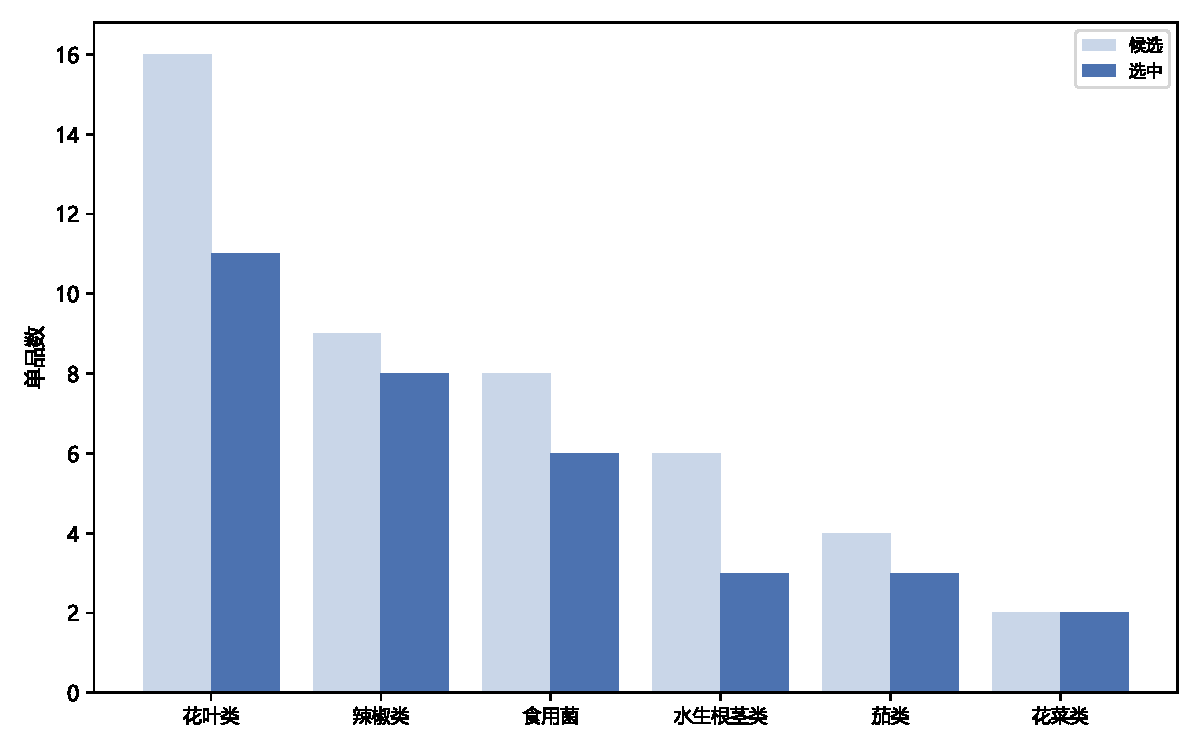
\includegraphics[width=0.8\linewidth]{figures/q3_selection.pdf}
\caption{候选与选中单品的分品类构成（柱状图，浅色为候选、深色为选中）}
\label{fig:q3_selection}
\end{figure}

分品类汇总见表 6。

\begin{table}[htbp]
\centering
\caption{分品类决策汇总}
\label{tab:q3_by_category}
\begin{tabular}{l r r r r r r r}
\toprule
品类 & 选中数 & 订购量合计（kg） & 可售量合计（kg） & 销量（kg） & 需求（kg） & 毛利合计（元） & 毛利占比 \\
\midrule
花叶类 & 11 & 124.03 & 111.20 & 111.20 & 111.20 & 201.99 & 29.6\% \\
辣椒类 & 8 & 81.35 & 74.18 & 73.76 & 73.76 & 220.56 & 32.3\% \\
食用菌 & 6 & 43.89 & 42.60 & 42.60 & 42.60 & 91.30 & 13.4\% \\
花菜类 & 2 & 15.90 & 14.42 & 14.42 & 14.42 & 80.11 & 11.7\% \\
茄类 & 3 & 17.82 & 16.74 & 16.74 & 16.74 & 58.56 & 8.6\% \\
水生根茎类 & 3 & 13.85 & 12.06 & 11.43 & 11.43 & 29.55 & 4.3\% \\
合计 & 33 & 296.83 & 271.19 & 270.14 & 270.14 & 682.08 & 100.0\% \\
\bottomrule
\end{tabular}
\end{table}

主要结果解读：
\begin{itemize}
    \item \textbf{选品结构}：最优解取到选品数上界 33 个，6 个品类全部覆盖；
    \item \textbf{满足率}：总体与各品类满足率均为 1.00；
    \item \textbf{利润来源}：辣椒类（220.56 元）与花叶类（201.99 元）合计占 62%，小米椒(份) 单品毛利 109.49 元；
    \item \textbf{定价行为}：弱弹性单品售价落在网格上界附近，弹性充分单品（西峡花菇 -2.52）取参考档 24.00 元/kg。
\end{itemize}

图 2 展示售价—订购量散点。

\begin{figure}[htbp]
\centering
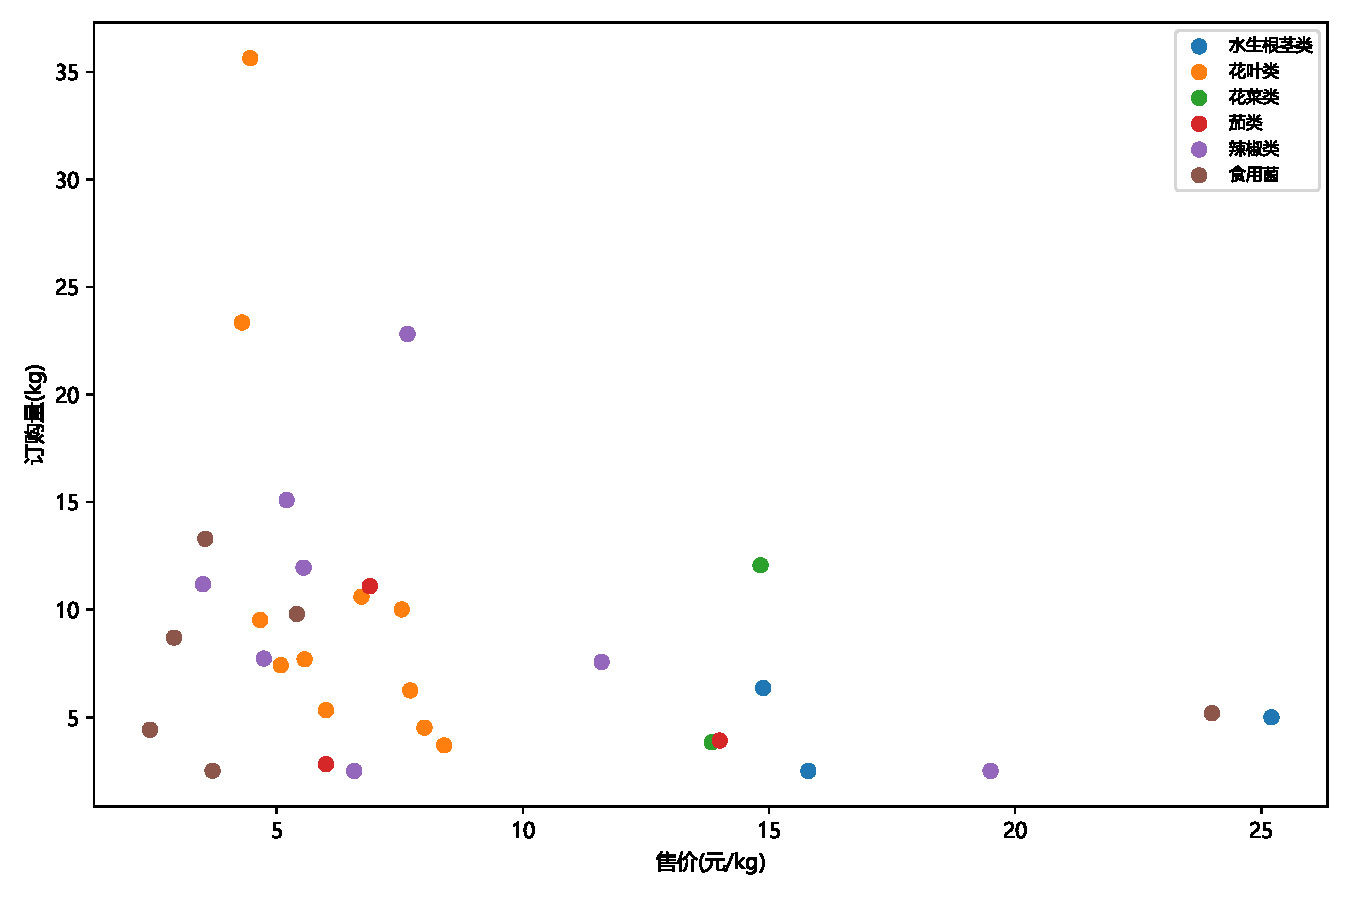
\includegraphics[width=0.8\linewidth]{figures/q3_price_qty.pdf}
\caption{选中单品售价—订购量散点（按品类着色）}
\label{fig:q3_price_qty}
\end{figure}

\subsubsection{决策时序与操作含义}

策略执行分三步：① 确定候选集与弹性、生成网格；② 求解 MIP 得到上架清单、售价档位与订购量；③ 当日执行。定价基于 6/24--30 批发价锁定，若实际批发价偏离，毛利变化见第九章灵敏度分析。

\subsubsection{小结}

问题三建立了单品级选品、定价与补货联合优化框架。以 45 个候选单品，在选品数 27--33、最小陈列量 2.5 kg 约束下，最优方案上架 33 个单品，总利润 682.08 元，满足率 1.00。灵敏度分析详见第九章，结论稳健；与问题二交叉核对通过。操作层面应优先保障小米椒(份)、西兰花等高毛利单品备货。

\textbf{局限与展望}：
\begin{itemize}
    \item 单品需求独立假设，无替代效应 \cite{kok2007,vanryzin1999}；
    \item 确定性需求未考虑随机性，可升级为单品级报童 \cite{federgruen1999,petruzzi1999}；
    \item 净销量低估真实需求 \cite{agrawal1996}；
    \item 未按周末偏置上调基准需求，结果偏保守；
    \item 满足率为软惩罚，可改为硬约束或鲁棒选品 \cite{vanryzin1999,rusmevichientong2012}；
    \item 未考虑动态折扣 \cite{elmaghraby2003} 与品类角色差异 \cite{dhar2001}。
\end{itemize}
% 问题四
\section{问题四的模型建立与求解}

\subsection{问题分析}

问题四要求从优化蔬菜类商品补货和定价决策的角度出发，识别当前数据体系的不足，提出补充采集数据的建议，并论述这些数据对解决前述三个问题的具体帮助。

基于前三问的建模与求解过程，现有数据（附件1至附件4）存在以下五个方面的缺失，制约了各模型的进一步优化改进：

\begin{enumerate}
\item \textbf{日销量聚合口径无法区分共同趋势与真实关联。} 问题一中的Spearman相关系数基于日销量聚合计算，无法唯一识别购物篮层面的互补或替代关系。
\item \textbf{售价口径混合了正常销售与打折销售。} 附件2无法区分正常售价与傍晚清仓打折价，问题二中品类售价$P_{c,t}$为混合口径，导致价格弹性$\hat{\beta}_c$向零衰减。
\item \textbf{缺货日真实需求不可观测。} 附件2仅记录已售销量$Q_{i,t}$，问题三中基准需求$d_i$将系统性低估真实需求。
\item \textbf{损耗率为静态平均值，缺乏动态结构。} 附件4仅给出各商品近期的盘点周期平均损耗率$L_i$，问题二、三均假设损耗率恒定。
\item \textbf{数据粒度为日级别，缺少日内信息与外部参照。} 附件2为日粒度数据，无法支持日内动态调价；附件3缺少周边竞品零售价参照。
\end{enumerate}

基于上述诊断，本节从需求侧、市场侧、运营侧、供给侧与外部环境五个维度提出数据采集建议。


\subsection{数据采集建议}

\subsubsection{需求侧：真实会员ID与缺货登记日志}

\paragraph{采集内容}

在POS收银环节采集脱敏后的会员ID（或家庭户标识），建立跨期交易流水关联；同时，在收银台或线上小程序记录“消费者搜索但未找到”的缺货登记日志，记录单品$i$在日期$t$的缺货登记次数$m_{i,t}$。

\paragraph{模型帮助}

有了真实交易流水号后，可精准还原消费者的真实购物篮$\mathcal{B}_{m,t} = \{i : \text{会员 } m \text{ 在 } t \text{ 日购买了单品 } i\}$，直接开展购物篮关联分析，弥补问题一中仅能通过销量相关性刻画品类/单品关系的不足。计算单品$i$与$j$的提升度：
\begin{equation}
\text{Lift}(i \to j) = \frac{P(i \cap j)}{P(i)P(j)} = \frac{|\{m : i, j \in \mathcal{B}_m\}| / |\{m\}|}{\left(|\{m : i \in \mathcal{B}_m\}| / |\{m\}|\right) \left(|\{m : j \in \mathcal{B}_m\}| / |\{m\}|\right)}.
\end{equation}

当$\text{Lift}(i, j) > 1$时，$i$与$j$存在真实互补关系；$\text{Lift}(i, j) < 1$暗示替代关系。

利用会员ID可追踪消费者的跨期购买行为，将问题二、三中的“群体聚合幂律需求”升级为基于会员分层的需求模型（RFM分群+价格敏感度分层），实现分层差异化促销，而非“千人千面”个体定价（个人定价不现实且有合规风险）。

缺货登记数据可精确估计被抑制的真实需求。设真实需求满足：
\begin{equation}
D_{i,t}^* = Q_{i,t} + \alpha_i \cdot m_{i,t} + \varepsilon_{i,t},
\end{equation}
其中$\alpha_i$为单品$i$的缺货登记率，通过小规模抽样校准。直接修正问题三中单品基准需求$d_i$的估计偏差：
\begin{equation}
d_i^* = \frac{1}{T_{\text{win}}} \sum_{t \in \text{win}} \left[ Q_{i,t} + \alpha_i m_{i,t} \right],
\end{equation}
使报童模型中的$\mu_{c,t}$预测更为准确。

\paragraph{决策帮助}

补货量更贴近真实需求，降低缺货损失；按会员分层做差异化促销，兼顾利润与顾客留存；真实购物篮关联指导选品组合与关联陈列。

\paragraph{理由与可行性}

缺货登记近乎零成本（POS/小程序增加一个登记字段即可）；会员ID属中等改造成本，需做脱敏与隐私合规（《个人信息保护法》：最小化采集、匿名化、仅存聚合特征）。

\paragraph{偏误风险与验证}

风险：缺货登记可能重复/误报、会员数据稀疏。处理：按“会员+商品+时段”去重、设置最小登记量阈值；稀疏会员不做个体建模，仅聚合到分群。验证钩子：用缺货登记修正前后的$d_i$、$\mu_{c,t}$分别回测报童缺货率与利润，对比修正是否带来显著改善。


\subsubsection{市场侧：陈列拓扑图与竞品实时均价}

\paragraph{采集内容}

采集各蔬菜单品在货架上的物理位置坐标（空间距离矩阵），以及周边3公里内农贸市场、生鲜电商的同品类实时标价。

\paragraph{模型帮助}

问题三的需求函数$D_i(p)$假设单品需求彼此独立（仅通过品类覆盖约束软性关联），无法量化“小白菜涨价后消费者转向上海青”的替代效应。引入上述数据后，将问题三需求函数扩展为包含交叉价格弹性的形式：
\begin{equation}
D_i(p_i, \mathbf{p}_{-i}) = d_i \left( \frac{p_i}{p_i^0} \right)^{\beta_i} \prod_{j \ne i} \left( \frac{p_j}{p_j^0} \right)^{\epsilon_{ij}},
\end{equation}
其中$\epsilon_{ij}$为单品$i$对单品$j$价格的交叉弹性。$\epsilon_{ij}$通过历史价格变动事件估计，并依据货架距离$\text{dist}_{ij}$加权：
\begin{equation}
\epsilon_{ij} = \epsilon_{ij}^0 \cdot \exp(-\lambda \cdot \text{dist}_{ij}), \quad \lambda > 0.
\end{equation}
交叉弹性矩阵可直接嵌入问题三的MIP模型中，将目标函数中的$D_{i,k}$从单变量函数扩展为多变量耦合函数，使最优选品结果在替代品之间实现利润平衡，避免“同类相食（Cannibalization）”效应。当$\epsilon_{ij}=0$（$i\neq j$）时，式(4)自动退化为独立需求$D_i(p_i)=d_i(p_i/p_i^0)^{\beta_i}$，保证模型体系自洽。

引入竞品价格后，在定价约束中增设外部参照：
\begin{equation}
p_{i,k} \le (1 + \theta) \cdot P_{i,t}^{\text{comp}},
\end{equation}
其中$\theta$为商超相对竞品的可接受溢价率，由历史数据估计。

\paragraph{决策帮助}

定价考虑外部比价与内部替代，联合定价避免内部利润自相蚕食；陈列拓扑指导选品与货架布局，邻近替代品采用差异化定价。

\paragraph{理由与可行性}

现有附件无竞品数据，弹性估计存在竞争环境混淆；竞品价格可通过人工抽样或公开平台采集，成本中等，建议中期落地。

\paragraph{偏误风险与验证}

风险：竞品采样本底不一致、价格可比口径差异。处理：只对同口径价格建模、缺失用品类均值填充并打缺失标记。验证钩子：加竞品变量前后回归$R^2$与AIC对比；交叉弹性模型的选品利润与独立需求模型选品利润对比。


\subsubsection{运营侧：小时级库存水位与日内打折流水}

\paragraph{采集内容}

借助RFID或电子秤联网系统，采集日内分时段的库存余量与鲜度评级变化；同时记录黄昏清仓时段（如19:00后）的具体折扣率与对应销量（附件2已有“是否打折”标记，缺的是折扣率与时段，属低成本增量改造）；采集分时段客流量、客单价（可由收银小票聚合得到）。

\paragraph{模型帮助}

问题二、三假设每日为独立的“单周期报童问题”，未考虑日内价格随鲜度衰减的动态调整。引入上述时序数据后，可建立日内动态定价的随机控制模型。设每日分为$T$个时段，状态变量为$(I_\tau, g_\tau)$（$I_\tau$为剩余库存，$g_\tau$为品相等级），决策变量为折扣率$\delta_\tau$，值函数满足贝尔曼方程：
\begin{equation}
V_\tau(I_\tau, g_\tau) = \max_{\delta_\tau \in [0, \bar{\delta}]} \left\{ \mathbb{E}\left[ p(\delta_\tau)\min(D_\tau(p), I_\tau) + V_{\tau+1}\left(I_\tau - \min(D_\tau, I_\tau), g_{\tau+1}\right) \right] \right\},
\end{equation}
终端条件$V_T(\cdot, \cdot) = 0$。该模型确定各时段的最优折扣率，决定每日下午/傍晚的最优清仓时点与折扣梯度。

动态定价模型是对问题二、三中“固定日定价”策略的日内精细化补充（主模型仍是日定价，日内DP是补充层）。其输出的“预期日内折扣损失”可作为修正项，回传到报童模型的临界比$\kappa_{c,t}$中，避免因过度乐观定价导致晚间积压损耗。

\paragraph{决策帮助}

给出每日最优清仓时点与折扣梯度，平衡“晚间低价清货”与“利润损失”；补货量在临界比层面已预扣日内折价损失，减少期末报废。

\paragraph{理由与可行性}

打折流水为低成本增量改造（补折扣率与时段字段即可）；RFID/电子秤联网成本较高，作为长期可选项。

\paragraph{偏误风险与验证}

风险：时段库存测量噪声、鲜度评级主观、清仓折扣与正常售价混记。处理：鲜度评级用统一标准打分，折扣单单独标记。验证钩子：日内DP的期末损耗率与固定日定价回测对比；临界比修正前后的缺货率/报废率对比。


\subsubsection{供给侧：分环节损耗率与供应商履约指数}

\paragraph{采集内容}

按“运输 $\to$ 入库 $\to$ 上架 $\to$ 清仓”四个节点分段记录实际损耗率；同时追踪各供应商的历史到货提前期（LTD）及批次合格率；采集每日实时进货价与供应商报价（含波动区间）。

\paragraph{模型帮助}

问题二、三假设综合损耗率$L_i$在预测期内恒定（来自附件4）。引入分环节数据后，可将常数$L_i$拓展为基于历史分环节损耗率拟合的时变衰减函数。设单品$i$批次$v$在储存$\tau$小时后的环节$s$损耗率为：
\begin{equation}
L_{i,v}^{(s)}(\tau) = L_{i,0}^{(s)} \cdot \exp(\lambda_s \tau) \cdot \left(1 - \frac{\eta_{i,v}}{5}\right),
\end{equation}
其中$\lambda_s > 0$为环节$s$的损耗加速因子，由历史分环节损耗数据拟合得到，$\eta_{i,v}$为批次鲜度评分。综合损耗率为：
\begin{equation}
L_{i,v}(\tau) = 1 - \prod_{s=1}^{4} \left(1 - L_{i,v}^{(s)}(\tau)\right).
\end{equation}
时变损耗函数可替代问题二中的固定损耗放缩因子$1/(1-L_c)$，将补货量$R_{c,t}$的计算升级为：
\begin{equation}
R_{c,t} = \frac{\mu_{c,t}(P^*) + \Phi^{-1}(\kappa_{c,t}) \cdot \sigma_{c,t}(P^*)}{1 - \bar{L}_{c,t}},
\end{equation}
其中$\bar{L}_{c,t} = \sum_{i \in \mathcal{C}_c} w_i \cdot L_{i,v(t)}(\tau_t)$，$v(t)$为$t$日的供应批次编号，$\tau_t$为截止补货决策时该批次已储存的时长。

提前期不确定性引入安全库存项（需求率$\mu_d$、提前期标准差$\sigma_L$）：
\begin{equation}
\text{SS} = z \cdot \sqrt{\sigma_d^2 \cdot L + \mu_d^2 \cdot \sigma_L^2}.
\end{equation}
实时批发价可将“未来一周批发价取最近均价”的假设升级为价格情景区间，支撑灵敏度分析。

\paragraph{决策帮助}

补货量同时反映“到货品质批次差异”和“上架后随时间衰减”的双重不确定性，显著提升报童模型在恶劣供应链条件下的抗风险能力；供应商履约指数可指导供应商选择与订货量分配。

\paragraph{理由与可行性}

分环节损耗需门店交接单改造，成本中低，建议短期优先；供应商履约数据需与供货方对接，属中期项。

\paragraph{偏误风险与验证}

风险：环节归属不清、提前期样本少。处理：交接单逐节点签字确认损耗责任；提前期至少收集10个批次再启用安全库存公式。验证钩子：时变损耗与恒定损耗的期末损耗率回测对比；含/不含提前期安全库存的缺货率对比。


\subsubsection{外部环境：天气、节假日与促销日历}

\paragraph{采集内容}

接入日/小时级天气数据（温度、降水量、湿度、极端天气哑变量）；整理节假日、节气、周末与大型活动日历；记录商超自身促销活动计划（促销品类、折扣力度、起止时间）。

\paragraph{模型帮助}

天气与节假日是蔬菜需求最强的外生驱动因素（4–10月供给丰富、极端天气推高叶菜需求），直接进入问题二的需求—价格回归与Prophet预测，作为外生回归项：
\begin{equation}
\begin{split}
\ln Q_{c,t} = \;&\alpha_c + \beta_c\ln P_{c,t} \\
&+ \sum_{k=1}^{6}\delta_k\mathbf{1}_{\{\text{weekday}=k\}}
+ \sum_{m=1}^{11}\eta_m\mathbf{1}_{\{\text{month}=m\}}
+ \gamma_T T_{c,t} + \gamma_R R_{c,t} \\
&+ \theta_1 \text{Holiday}_t + \theta_2 \text{Promo}_t + \varepsilon_{c,t},
\end{split}
\end{equation}
其中$T_{c,t}$为温度，$R_{c,t}$为降水量，$\text{Holiday}_t$为节假日哑变量，$\text{Promo}_t$为促销哑变量。

引入这些变量后，可剔除天气和促销活动对销量的干扰，使$\hat{\beta}_c$的估计更加准确；同时提升Prophet预测中基准需求$\bar{Q}_{c,t}$与残差标准差$\sigma_{c,t}$的精度，改善报童补货量的均值—方差结构。

\paragraph{决策帮助}

预测期若遇极端天气或节假日，自动上调补货量与价格保护区间；促销日历与定价联动，避免促销期与非促销期需求混淆导致弹性误估。

\paragraph{理由与可行性}

成本极低（公开API+内部日历），见效最快，建议最高优先级。

\paragraph{偏误风险与验证}

风险：天气数据粒度不一致、促销与需求互为因果。处理：用门店最近气象站数据；促销变量只用于“去混淆”，弹性估计以非促销样本为主或加入促销交互项。验证钩子：加天气/促销变量前后Prophet回测RMSE与MAE对比。


\subsection{综合分析}

\subsubsection{数据—模型—决策对应总览}

\begin{table}[htbp]
\centering
\caption{数据—模型—决策对应关系}
\label{tab:mapping}
\begin{tabular}{cccc}
\toprule
数据类别 & 影响的前问模型/参数 & 改善的决策 & 实施成本 \\
\midrule
会员ID/购物篮 & Q1 关联分析 & 选品组合、关联陈列 & 中 \\
缺货登记 & Q2 $\mu_{c,t}$、Q3 $d_i$ & 补货量、缺货率 & 低 \\
会员分层 & Q2 需求分层、Q3 单品需求 & 分群促销 & 中 \\
竞品实时均价 & Q2 $\beta_c$校准、Q3 $\epsilon_{ij}$ & 联合定价 & 中 \\
陈列拓扑 & Q3 替代/互补结构 & 货架布局、选品 & 中 \\
日内库存/鲜度 & Q2/Q3 $\kappa_{c,t}$、日内DP & 清仓时点、折扣梯度 & 高 \\
日内打折流水 & Q2/Q3 $\kappa_{c,t}$ & 清仓折扣、期末报废 & 低 \\
分时段客流 & Q2 日内需求估计 & 排班、促销时段 & 中高 \\
分环节损耗率 & Q2/Q3 $L_i \to \bar{L}_{c,t}$ & 补货量、报废率 & 中低 \\
供应商履约 & Q2 安全库存 & 供应商选择 & 中 \\
实时批发价 & Q2 $W_{c,t}$情景化 & 定价调整 & 中低 \\
天气/节假日 & Q2 回归/Prophet外生项 & 补货与价格预警 & 极低 \\
促销日历 & Q2 弹性去混淆 & 促销与定价联动 & 低 \\
\bottomrule
\end{tabular}
\end{table}

\subsubsection{实施优先级与ROI评估}

五类数据在采集成本和模型改进效果上存在差异。采集价值可量化为“决策增益 − 采集成本”：P1类数据（天气、缺货登记、促销日历、分环节损耗）总改造成本最低，而预期缺货/报废率下降带来的毛利提升通常远高于成本，短期投入回报为正。优先级排序见表\ref{tab:priority}。

\begin{table}[htbp]
\centering
\caption{五类数据采集方案的优先级排序}
\label{tab:priority}
\begin{tabular}{ccccc}
\toprule
优先级 & 数据维度 & 数据方案 & 采集方式 & 实施成本 \\
\midrule
1 & 外部环境 & 天气、节假日与促销日历 & API接入+内部排期表 & 极低 \\
2 & 需求侧 & 会员ID+缺货登记 & POS系统改造+收银台登记 & 中 \\
3 & 运营侧 & 折扣标记+分时段库存 & POS/电子秤系统升级 & 低 \\
4 & 供给侧 & 分环节损耗率+供应商评级 & 验收流程+PDA录入 & 中 \\
5 & 市场侧 & 货架位置+竞品均价 & 平面测绘+数据采集 & 高 \\
\bottomrule
\end{tabular}
\end{table}

\subsubsection{数据间的协同效应}

五类数据并非独立发挥作用：

\begin{enumerate}
\item 天气/促销日历与折扣标记结合：天气和促销日历可作为外生变量辅助区分“促销导致的销量变化”与“正常需求波动”，使折扣标记$r_{i,t}$的分层弹性估计更加准确；
\item 折扣标记与缺货登记结合：折扣标记$r_{i,t}$刻画价格降低对销量的影响，缺货登记$m_{i,t}$刻画价格过低导致缺货时被抑制的需求，二者共同覆盖需求函数$D_i(p)$的可观测区间两端；
\item 购物篮关联与货架距离结合：购物篮关联$\text{Lift}(i,j)$与货架距离$\text{dist}_{ij}$结合，可估计空间距离对替代弹性的衰减因子$\lambda$；
\item 分时段库存与分环节损耗率结合：分时段库存$I_{i,t,\tau}$与分环节损耗率$L_{i,v}^{(s)}(\tau)$结合，损耗率随时间加速增长的函数关系可直接嵌入贝尔曼方程的状态转移。
\end{enumerate}

\subsection{小结}

问题四从需求侧、市场侧、运营侧、供给侧与外部环境五个维度提出了五类补充数据的采集方案，分别对应前三个模型的关键局限：

\begin{enumerate}
\item 需求侧——会员ID与缺货登记：解决问题一销量相关无法识别真实购物篮关联的问题，修正问题三因缺货截断导致的需求低估；
\item 市场侧——陈列拓扑与竞品均价：为问题三引入交叉价格弹性和外部竞争定价约束，弥补独立需求假设的不足；
\item 运营侧——日内库存与打折流水：解决问题二价格弹性估计中混合口径导致的衰减偏误，并将日清报童扩展为日内动态定价；
\item 供给侧——分环节损耗率与供应商评级：将问题二、三的恒定损耗率替换为基于批次品质和储存时长的动态损耗函数；
\item 外部环境——天气、节假日与促销日历：提升需求预测精度，剔除促销和天气对弹性估计的干扰。
\end{enumerate}
% 模型的分析与检验（精简版：正文仅保留检验契约汇总表；其余 6 表与 1 图的环境移至文末"附录图表"块，排版时请移入正式附录，正文 \ref 编号不变）
\section{模型的分析与检验}

为检验结论的可信度及其成立条件，本章从灵敏度分析与模型检验两个层面展开验证：灵敏度分析通过对由数据估计或人为设定的关键参数施加合理扰动，考察最优决策与目标值是否发生量级性变化 \cite{saltelli2008}；模型检验则从分布诊断、样本外回测、基线对比、随机模拟与求解器状态校验等方面，检验模型假设、估计精度与求解可靠性。所有判定阈值均在运行前声明，检验契约（claim--perturbation--metric--threshold--observed--status）固化于 \texttt{q2\_robustness\_summary.json}，状态取 PASS 或 CONDITIONAL（边界在正文注明）；数值均可追溯至对应 CSV 与脚本（\texttt{A.py}--\texttt{D.py}、\texttt{q2\_sensitivity.py}、\texttt{q3.py}），随机模拟固定种子 SEED=7、每组样本量 $N=20000$，以保证可复现性。量级稳定判据为：利润与补货量扰动分别不超过 30\% 与 20\%，回测 MAPE 不超过 40\%，相关模拟期望利润偏差不超过 1\%。

\subsection{灵敏度分析}
\label{sensitivity_analysis}
\subsubsection{问题一：网络阈值与聚类稳定性}

相关系数阈值取 0.3、0.4、0.5 时，主边数分别为 1848、1062、523 条，稳健边数分别为 249、154、81 条（表~\ref{tab:threshold}，见附录），边数随阈值单调下降、正负边占比方向稳定，表明“品类/单品间以正相关为主、少数负相关”的结构性结论不依赖于阈值选择；主口径 0.4 下 154 条稳健边构成 51 节点协同变动网络。聚类簇数扫描中，silhouette 系数在 $k=5$ 处取得最大值 0.2583，超过 0.15 的选取下限（表~\ref{tab:silhouette}，见附录）；对 132 个单品做 80\% 抽样并重复聚类 50 次 \cite{efron1993}，平均调整兰德指数 ARI=0.4567，聚类结构中等稳定，且聚类标签与全样本独立重算的 Ward 聚类完全一致（特征最大偏差约 $10^{-14}$）。

\subsubsection{问题二：定价与补货参数灵敏度}

对批发价、价格弹性、价格口径与损耗率四类关键输入施加扰动，统一以未来一周总补货量与总期望利润为口径（表~\ref{tab:q2_sensitivity}、图~\ref{fig:q2_sensitivity}，见附录）：

\begin{itemize}
    \item \textbf{批发价 $\pm10\%$}：总补货量变化约 $\pm5\%$，总利润变化 +0.3\%/−0.7\%，均小于 1\%，定价与补货策略稳健（PASS）；
    \item \textbf{弹性 $\pm20\%$}：各品类弹性绝对值在 $\pm20\%$ 扰动后最大约 0.60，最优加价率与售价保持不变，总利润变化 −0.4\%/+0.5\%（PASS）；
    \item \textbf{价格口径切换}：当期销售额加权口径下弹性符号不变、绝对值普遍增大，利润 +26.7\%，与主口径机制一致；中位价口径下水生根茎类、食用菌弹性符号翻转、利润虚高 +72.8\%，该口径不可采用（CONDITIONAL）；
    \item \textbf{损耗率替换}：以 2022-07 至 2023-06 单品销量份额加权损耗率替代固定基期份额 $L_c=\sum_i w_i L_i$，利润 +7.5\%、补货量 −1.0\%，量级不变（PASS）。
\end{itemize}

\subsubsection{问题三：组合优化灵敏度}

对缺货惩罚、选品数、弹性、批发价、损耗率、价格网格与大 M 七类设定逐一重解 MIP（表~\ref{tab:q3_sensitivity}，见附录），全部情景求解状态 optimal、最优性 gap=0。缺货惩罚 $\rho$（0.5--1.5）与大 M 放大 50\% 情景的最优解完全不变：前者因基准方案无缺货、惩罚项不进入目标值，后者结合订购量上界余量检查（最小余量 12.58 kg）确认可行域未被截断。选品数 27/30/33 对应利润 657.54/673.60/682.08 元；弹性 $\pm20\%$ 使利润变化 −1.6\%/+1.7\%，方向与问题二一致；批发价 $\pm10\%$ 为最敏感输入（利润 −17.6\%/+18.1\%），且 $\times1.1$ 时 1 个低毛利单品被挤出；损耗率取分类级时利润 −3.6\%；价格网格 $K=7$ 与分位数取点分别使利润 −3.7\%/+4.5\%，离散化影响控制在 $\pm5\%$ 以内。

\subsection{模型检验与误差分析}

\subsubsection{问题一：分布、季节与关联结构检验}

六品类日销量按 AIC 选型为伽马（4 个）与对数正态（2 个），BIC 交叉核对一致，QQ 图无系统性偏离（图文件：\texttt{q1\_dist\_cat\_qq.pdf}）；K-S 检验在参数估计后偏保守，仅作图形诊断。STL 分解的季节强度 0.1729--0.2616、趋势强度 0.5135--0.6268，与独立重算最大偏差 $5\times10^{-5}$。协同网络主边 1062 条中 154 条通过前后半样本检验成为稳健边，抽样 200 条边独立重算的相关系数最大偏差 $5\times10^{-5}$，FDR $q$ 值与标准 BH 校正一致；聚类抽样稳定性 ARI=0.4567（见 9.1.1）。

\subsubsection{问题二：需求—价格模型、预测与报童检验}
\label{stability_q2}
回归诊断表明，六品类价格弹性 $t$ 值分别为 −6.79、−5.45、−0.70、−3.16、−3.03、−5.28，除水生根茎类（$t=-0.70$）外均在 1\% 水平显著，该品类定价结论相应降级（详见表~\ref{tab:q2_elasticity}）；$R^2$ 介于 0.31--0.61，$\ln P$ 相关矩阵条件数为 7.9，不存在严重共线性（图文件：\texttt{q2\_elasticity\_fit.pdf}）。

样本外回测以 MAPE 度量，求和仅对实际销量 $Q_t>0$ 的日期进行：
\begin{equation}
\mathrm{MAPE}=\frac{100\%}{n}\sum_{t}\frac{\left|\hat Q_t-Q_t\right|}{Q_t}.
\end{equation}
后 28 天滚动回测 MAPE 为 20.6\%--37.2\%；2022-07 同期回测为 23.9\%--66.4\%，除辣椒类外各品类误差均高于后 28 天口径，最大 66.4\%（茄类）超过 40\% 阈值（CONDITIONAL），表明跨年外推稳定性有限，2023-07 预测区间应保守解读（表~\ref{tab:backtest}，见附录；数据文件：\texttt{q2\_backtest.csv}、\texttt{q2\_backtest\_2022.csv}）。

基线对比中，报童最优分位数订货相对确定性补货 $R^0_{c,t}=\mu_{c,t}(P^*)/(1-L_c)$ 的总期望利润为 5305.19 vs 4550.45 元（增益 +754.74 元），总补货量 2607.89 vs 3190.54 kg（低 18.3\%），日均缺货率 0.51--0.80 vs 0.39--0.43，体现“少订少损耗换更高期望利润”的最优取舍；水生根茎类在确定性口径下利润为负（−112.79 元）、报童口径转正（360.99 元），与其临界比最小（$\kappa=0.20$）一致（表~\ref{tab:nv_det}，见附录；数据文件：\texttt{q2\_nv\_det.csv}）\cite{han2026}。

品类相关联合模拟以残差 Pearson 相关矩阵（非对角元 0.24--0.74）构造高斯 copula \cite{nelsen2006}，配合对数正态边际模拟每日 2 万组（SEED=7）：相关口径期望利润 5311.26 vs 独立口径 5305.19 元（+0.11\%，在 1\% 阈值内，PASS），方差比 2.47，证实“相关性只进入方差、不进期望”（数据文件：\texttt{q2\_joint\_sim.csv}）。

\subsubsection{问题三：求解可靠性与可行性检验}

基准及全部灵敏度情景求解状态 status=0、最优性 gap=0，五项约束逐条校验通过（选品数 33 $\in$ [27,33]、最小陈列量 2.5 kg、可售量 $\le$ 订购量 $\times(1-L_i)$、价格在网格内、品类全覆盖）（数据文件：\texttt{q3\_diagnostics.csv}）；3 个低需求单品因最小陈列约束超订 1.16 kg（成本 10.53 元）已计入成本。大 M 取值 $\max(3\max_t Q_{i,t}^{\mathrm{hist}},\ 2.5,\ 1.05D_{i,1})$ 的最小余量 12.58 kg，放大 50\% 后最优解不变，双重确认可行域未被截断（数据文件：\texttt{q3\_mbound.csv}）。跨问题交叉核对中，问题三各品类可售量加总 $\sum_{i\in\mathcal{C}_c}q_i(1-L_i)$ 与问题二品类期望需求 $\mu_{c,t}(P^*)$ 之比为 0.21--0.74，量级同阶、结构一致，差异源于计划层级与约束口径，属预期差异而非矛盾（数据文件：\texttt{q3\_vs\_q2.csv}）。

\subsubsection{检验结论汇总}

七项量化检验的契约见表~\ref{tab:summary}：5 项 PASS、2 项 CONDITIONAL（中位价口径不可采用、2022-07 跨年回测误差更高），相应边界已在正文标注；主结论在参数扰动、口径替换、基线对比与随机模拟下保持稳健。

\begin{table}[htbp]
\centering
\caption{模型检验契约汇总（阈值运行前声明）}
\label{tab:summary}
\begin{tabular}{l l r r l}
\toprule
检验项 & 扰动/方法 & 阈值 & 观测值 & 状态 \\
\midrule
批发价 $\pm10\%$ 利润稳定 & $W\times1.1$、$W\times0.9$ & $\le30\%$ & 0.7\% & PASS \\
弹性 $\pm20\%$ 决策稳定 & 品类弹性 $\times1.2$、$\times0.8$ & $\le30\%$ & 0.5\% & PASS \\
价格口径切换 & 固定权重→当期加权/中位价 & $\le30\%$ & 72.8\% & CONDITIONAL \\
报童优于确定性 & 最优分位数 $y^*$ vs 均值 & 利润差 $\ge0$ & +754.74 元 & PASS \\
损耗率替换 & 固定份额→单品销量加权 & 补货变化 $\le20\%$ & 1.0\%（补货量） & PASS \\
2022-07 同期回测 & 样本截止 2022-06-30 & MAPE $\le40\%$ & 66.4\% & CONDITIONAL \\
品类相关联合模拟 & 残差相关 vs 独立（高斯 copula） & 利润偏差 $\le1\%$ & 0.11\% & PASS \\
\bottomrule
\end{tabular}
\end{table}

\subsubsection{模型局限（三问共享）}

缺货日销量截断使需求与弹性估计轻微低估；水生根茎类弹性不显著（$t=-0.70$），其定价结论证据不足；跨年（2022-07）预测误差高于后 28 天口径，外推至 2023-07 应保守。

\subsection*{本章小结}

三问结论在灵敏度与模型检验下量级稳定：问题一结构结论不依赖阈值选择、聚类 ARI=0.4567；问题二批发价与弹性扰动下利润变化均小于 1\%，报童增益 +754.74 元，相关模拟证实“相关性只进入方差、不进期望”（偏差 +0.11\%，方差比 2.47）；问题三全部情景 optimal 且约束通过，批发价为最敏感输入（约 $\pm18\%$）、网格离散化影响约 $\pm4.5\%$。七项检验 5 项 PASS、2 项 CONDITIONAL，在标注的两项边界条件下，模型结论可作为商超补货定价决策的依据。
% 模型评价、改进与推广
\section{模型的评价、改进与推广}
\subsection{模型的优点}
\begin{itemize}[itemindent=2em]
  \item 优点1：待写。
  \item 优点2：待写。
\end{itemize}

\subsection{模型的缺点}
\begin{itemize}[itemindent=2em]
  \item 缺点1：待写。
\end{itemize}

\subsection{模型的改进}
待写。

\subsection{模型的推广}
待写。


% ================= AI 工具使用声明 =================
\section*{AI 工具使用声明}
本参赛队在竞赛过程中使用了AI 工具，主要用于论文语言润色与排版、部分文献与建模方法初步查找；最终方法的选取、模型建立、代码编写均由参赛队人工完成。详细使用情况见支撑材料。

% ================= 参考文献 =================
\clearpage
% \nocite{*}  % 如需列出 ref.bib 中所有条目，取消注释；平时用 \cite{key} 引用
\bibliographystyle{gbt7714-numerical}
\bibliography{ref}

% ================= 附录 =================
\clearpage
% 附录：代码清单、中间数据说明等
\begin{appendices}

\section{文件清单}
\begin{table}[H]
  \centering
  \begin{tabularx}{\textwidth}{LL}
    \toprule
    文件名 & 功能说明 \\
    \midrule
    code/xxx.py & 待写 \\
    \bottomrule
  \end{tabularx}
  \caption{程序文件清单}
  \label{tab:文件清单}
\end{table}

\section{关键代码}
% 示例：\lstinputlisting[language=python]{code/xxx.py}

\end{appendices}


\end{document}
